% Just use beamer, not ctexbeamer, if you're not typesetting Chinese
% \documentclass{beamer}
\documentclass[linespread=1.4,t]{ctexbeamer}

\usepackage[size=a3,orientation=portrait,scale=1.4]{beamerposter}

% (Mirage theme already loads fontawesome5)
\usetheme{Mirage}
% \usetheme[light]{Mirage}

% fonts
\usepackage[lining,tabular]{carlito}
\usepackage{caladea}
\usepackage{unicode-math}
\setmathfont{Erewhon Math}


% beamer slides -> poster = some adjustments needed
\setbeamerfont{headline}{size=\huge}
\setbeamerfont{footline}{size=\large}
\setbeamercolor{bibliography item}{fg=block body.fg}
\setbeamercolor{bibliography entry author}{fg=block body.fg}
\setbeamercolor{bibliography entry title}{fg=block body.fg}
\setbeamercolor{bibliography entry location}{fg=block body.fg}
\setbeamercolor{bibliography entry note}{fg=block body.fg}
\setlength{\MirageGlowRadius}{0.5ex}

% _slightly_ more prominent colours for the headline... but not so much
\makeatletter
\ifMirage@light
  \setbeamercolor{section in head/foot}{fg=structure!80!MirageGray0}
  \setbeamercolor{page number in head/foot}{fg=structure!80!MirageGray0}
\else
  \setbeamercolor{section in head/foot}{fg=structure!90}
  \setbeamercolor{page number in head/foot}{fg=structure!90}
\fi
\makeatother
\setbeamerfont{title}{size=\Huge}
\setbeamerfont{author}{size=\large}
% might need some extra vertical space when using [t]
\addtobeamertemplate{headline}{}{\vspace*{1ex}}

% yes I've sinned by abusing and re-defining \insertnavigation to quickly
% insert the title and author in the headline...
\renewcommand*{\insertnavigation}[1]{\centering\vspace*{-1ex}%
    {\usebeamerfont{title}%
     \insertshorttitle[width=0.95\hsize,respectlinebreaks,center]\par}%
    \vspace*{0.5ex}%
    {\usebeamerfont{author}%
     \insertshortauthor[width=0.95\hsize,respectlinebreaks,center]\par}%
}


% adjust itemize/enumerate list indents if necessary
\setlength{\leftmarginii}{1.75em}
\setlength{\leftmarginiii}{2.5em}

\usepackage{graphicx}
\usepackage[style=numeric,natbib]{biblatex}
\addbibresource{sample-refs.bib}


\title{当蜃楼Mirage主题拿来做海报}
\author{作者甲、作者乙、作者丙}
\renewcommand{\MirageFootlineContents}{Dept of XX, Uni of YY, 某某大学,其它适合资讯}

\begin{document}

\begin{frame}

\begin{columns}[T]
\column{.47\textwidth}
\begin{block}{Introduction}

\begin{itemize}
    \item 看机械的白鸽\faDove{} 从空中飞过 
    \item 要如何点睛\faEye[regular] 它才堪称鲜活

\begin{enumerate}
    \item 数字的晨昏\faCloudSun{} 是否更缤纷\faCloudMoon
    \item 仿生的情人\faGrinHearts{} 是否更忠贞\faGrin*[regular]
\end{enumerate}

    \item 推开一扇门\faDoorOpen{} 还有万千重门\faDoorClosed{\small\faDoorClosed}{\footnotesize\faDoorClosed}{\scriptsize\faDoorClosed}{\tiny\faDoorClosed}
\end{itemize}

\end{block}

\begin{block}{那来自过去 古老的眼神}
    \begin{enumerate}
        \item 如何能辨认 此刻是幻是真
        \begin{enumerate}
	        \item 人造的天分 是否算慧根
	        \begin{enumerate}
		        \item 克隆的肉身 是否有灵魂
		        \item 永远在追问 却从来都没结论
	        \end{enumerate}
        \end{enumerate}
        \item \alert{Can it be real}
    \end{enumerate}
\end{block}

\begin{pullquote}
    Can it be real\\
    The world is a mirage
\end{pullquote}

\bigskip
    
\setbeamercolor{pullquote}{fg=MirageBlue}
\renewcommand{\MiragePullquoteOpen}{\hskip-.2\ccwd『}
\begin{pullquote}
在电幻的荒丘 寻真实的绿洲\\
渺小得如蜉蝣 也仰望着宇宙
\end{pullquote}

\column{.47\textwidth}
\begin{exampleblock}{算了我也不知道在写什么,do you?}
Now solve $x = \frac{-b \pm \sqrt{b^2 -4ac}}{2a}$. 对各位同学来说应该挑战不大。
\end{exampleblock}

\begin{alertblock}{算了我也不知道在写什么,do you?}
\[ x = \frac{-b \pm \sqrt{b^2 -4ac}}{2a}, \quad\therefore \alpha \neq \Omega \]
\end{alertblock}

\begin{block}{算了我也不知道在写什么,do you?}
\[ x = \frac{-b \pm \sqrt{b^2 -4ac}}{2a}, \quad\therefore \alpha \neq \Omega \]
\end{block}

\begin{proof}
显而易见,$1+1=2$.
\end{proof}

\begin{theorem}
有一件很美好的事情将要发生,它终会发生。
\end{theorem}

\begin{definition}
有一件很美好的事情将要发生,它终会发生。
\end{definition}

\end{columns}

\begin{block}{Superior Images and False Horizons \citep{Mirage-Greenler1980,AtmRefrac-Hyperphysics}}
\begin{center}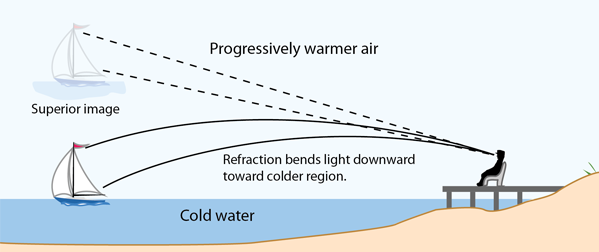
\includegraphics[width=0.95\hsize]{miragesup.png}\end{center}
% locally change the linespread for this English-only paragraph.
\linespread{1}\selectfont
A superior image can be produced when warm air exists over cold water. Again, using the pattern from Greenler, the vertical scale and the curvature are greatly exaggerated to show the effect. Such images are often seen at great distances in the arctic region when the air is significantly warmer than the water. Since the geometry of the mirage images depends on the details of the temperature contour, a great variety of mirage images can be formed.

Source: \url{http://hyperphysics.phy-astr.gsu.edu/hbase/atmos/mirage.html}
\end{block}

\vfill

\begin{block}{\refname}
% All English refs, so...
\renewcommand*{\bibfont}{\relsize{-1}\linespread{1}\selectfont}
\setlength{\biblabelsep}{0.25em}
\printbibliography[heading=none]
\end{block}

\end{frame}
\end{document}
